
\chapter{Autonomie}
\label{chap:autonomie}


\section{Kurze Einführung ins Segeln}
Bevor man Segelboote Autonom machen kann, muss man erst grob verstehen, wie diese sich Fortbewegen. 
\subsection{Segelstellungen}
Grundsätzlich unterscheidet man in 5 Kurse bzw. Segelstellungen.
\begin{itemize}
    \item Vorwind: Wenn der Wind von Hinten kommt. (\textbf{U})
    \item Im wind: Wenn der Wind von Vorne kommt.
    \item Halbwind: Wenn der Wind von $\pm$ 90$^{\circ}$ zum Boot kommt. (\textbf{U})
    \item Raumschot: Wenn der Wind schräg von hinten kommt. (\textbf{S})
    \item Vorwind: Wenn der Wind schräg von vorne kommt. (\textbf{S})
\end{itemize}
% TODO Bild von Segelstellungen

Davon sind alle ausser \textit{Im Wind} besegelbaar. Dies liegt daran, dass wenn der Wind von vorne kommt, dieser nicht vom Segel aufgefangen wird. Dieser Bereich wird als \textit{No Go Zone} bezeichnet und ist je nach Boot $\approx 90^{\circ}$. Auf den anderen Kursen wird das Boot entweder durch das Stossprinzip (\textbf{S}) angetrieben oder durch Umstörmung (\textbf{U}) was sehr Ähnlich wie bei Flügeln von Flugzeugen oder Rotorblättern von Windrädern funktioniert.  
\subsection{Wind}
Es ist Wichtig zwischen dem wahren Wind und dem scheinbaren Wind zu unterscheiden. Der wahre Wind kommt aus der echten Richtung. Wenn man auf die Messdaten eines Stationären Windsensors schaut, wird man den wahren Wind ablesen können. Der Scheinbare Wind hingegen ist ein Zusammensetzung aus dem wahren Wind und dem Fahrtwind. Wenn im Segeln von der Windrichtug gesprochen wird, meint man in der Regel den scheinbaren Wind, da miest nur dieser von Bedeutung ist. 
% TODO Vektor bild mit beiden Pfielen

\section{Software Architektur}
\subsection*{Betriebsystem}
Der Raspberry Pi, welcher für die Autonomie zuständig ist, wird mit der Raspberry Pi OS Linux Distribution betrieben. Linux hat im Gegensatz zu Arduinos, ESPs, etc. hat es den entscheidenden Vorteil, dass es einfach zu bedienen, zu warten und zu erweitern ist. Ebenfalls lässt es sehr einfach über WLAN Fernwarten. 

\subsection*{Docker}
Alle für das Boot geschriebenen Programme laufen in Dockercontainer. Docker ist eine Containerisierungstechnologie, welche es erlaubt, Anwendungen in isolierten Containern virtualisiert auszuführen. Diese Container sind leichtgewichtig und portabel.

\subsection*{Programmiersprache}
Aufgrund des einfachen Prototypen wurde die Prgrammiersprache Python gewählt. Im gegensatz zu sprachen wie C++ oder Rust welche um ein vielfaches performanter wären ist Python sehr langsam. Da die Algorithmen wie später nicht erläuter wird, nicht besonders Komplex sind, macht dies keinen Bedeutenden Unterschied. 


\section{Navigation}
Für dieses Projekt wurde sich für ein Wegpunkte basiertes System entscheiden. Somit gibt es einen klar definierten Anfangspunkt und einen klar definierter Endpunkt. Dies hat den Vorteil, dass so Bereiche welche besonders interessant sind sicher besucht werden, da der genaue weg aufgrund von den limitationen des Segelns nicht im Vorhinein definiert werden kann. \\
Daher muss ein Algorithmus entwickelt werden, welcher trotz Gegenwind einen Punkt erreichen kann. Der folgende Algorithmus wird im Anschluss genauer erläutert

\begin{algorithm}
\caption{Berechne neuen Kurs}
\begin{algorithmic}[1]
\Function{BerechneNeuenKurs}{$\vec{v}_{\text{Boot}}, \vec{v}_{\text{Wind}}, \vec{v}_{\text{Ziel}}$}
    \State $\text{Skalarprodukt} \gets \vec{v}_{\text{Wind}} \cdot \vec{v}_{\text{Boot}}$
    
    \State $\vec{neuerKurs} \gets \vec{v}_{\text{Ziel}}$
    
    \If{$\text{Skalarprodukt} < -0.8$}
        \If{$\vec{v}_{\text{Wind}} \cdot \vec{v}_{\text{Ziel}} > -0.8$}
            \State $\vec{neuerKurs} \gets \vec{v}_{\text{Ziel}}$
            \State \Return \Call{Normalisiere}{$\vec{neuerKurs}$}
        \EndIf
        
        \State $n \gets 0$
        \While{$\vec{v}_{\text{Wind}} \cdot \vec{neuerKurs} < -0.8$ \textbf{und} $n < 1$}
            \State $n \gets n + 0.1$
            \State $\vec{neuerKurs1} \gets \vec{v}_{\text{Ziel}} + n \cdot \begin{bmatrix}0 & -1 \\ 1 & 0\end{bmatrix} \cdot \vec{v}_{\text{Ziel}}$
            \State $\vec{neuerKurs2} \gets \vec{v}_{\text{Ziel}} + n \cdot \begin{bmatrix}-1 & 0 \\ 0 & 1\end{bmatrix} \cdot \vec{v}_{\text{Ziel}}$
            
            \If{$\vec{neuerKurs1} \cdot \vec{v}_{\text{Ziel}} > \vec{neuerKurs2} \cdot \vec{v}_{\text{Ziel}}$}
                \State $\vec{neuerKurs} \gets \vec{neuerKurs1}$
            \Else
                \State $\vec{neuerKurs} \gets \vec{neuerKurs2}$
            \EndIf
        \EndWhile
        
        \State \Return \Call{Normalisiere}{$\vec{neuerKurs}$}
    \EndIf
\EndFunction
\end{algorithmic}
\end{algorithm}
 

\begin{figure}[H]
    \centering
    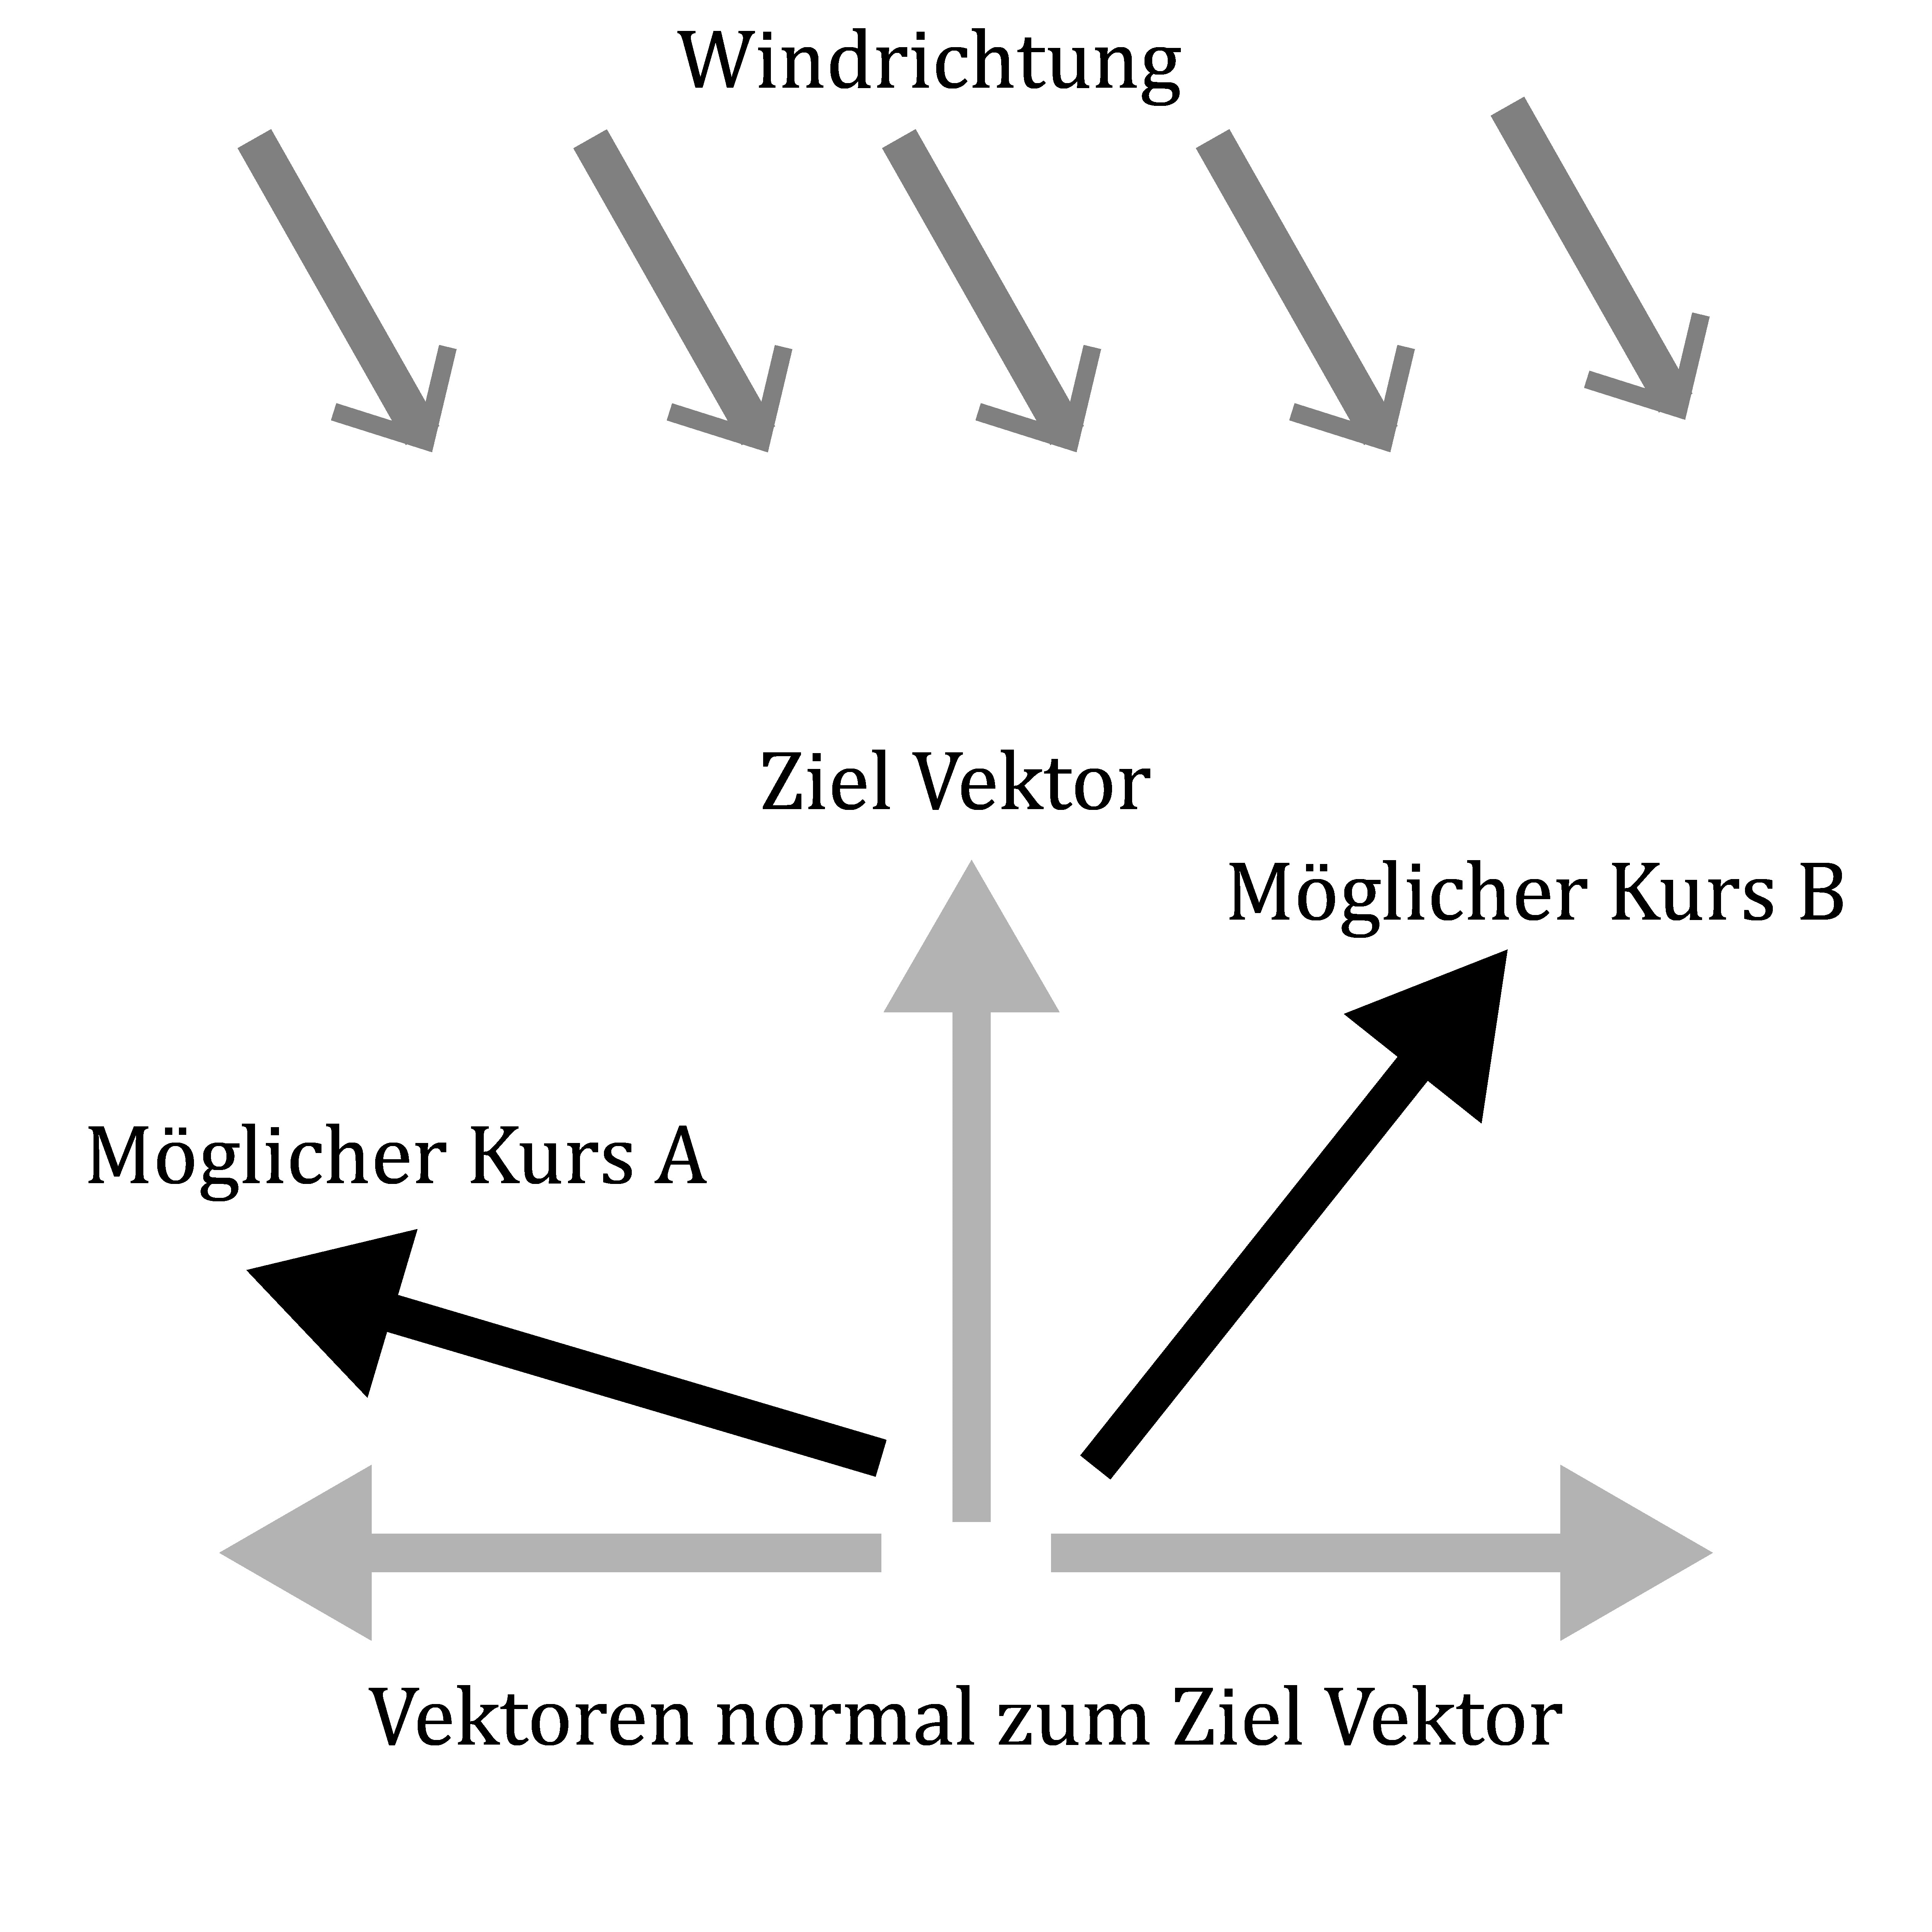
\includegraphics[width=0.5\linewidth]{algorythmus Vektoren.png}
    \caption{Visualisierung}
    \label{fig:enter-label}
\end{figure}




\section{Pathfinding}


\subsection{Deep reinforcment}
Der einzige Algorithmus aus der Familie des Maschinellen lernen ist Deep reinforcement. Da für das Training von ML algroythmen in de Regel umfangreiche Datensets verwenden müssen ist dies bedeutend schwer. Der Vorteil am Deep reinforcment ist dass dafür anfänglich keine Traingsdaten geben muss, da er sich diese durch "trail and error" selbst erlernt. Dafür muss eine virtuelle Umgebung geschaffen werden, wo man einem Roboter gewisse DOF gibt. Mit den gegeben Freiheiten wird versucht das gegebene Ziel möglichst Zeiteffizienz zu bewältigen. Trainiert wird es ganz ähnlich wie wir es von der Erziehung von Kindern kennen. Wenn die Neuronale Netz einen Fortschritt erreicht wird diese durch Punkte belohnt. Ganz im Gegenteil werden, bei Handlungen welche sich negativ auf das Ergebnis auswirken, Bestrafungen ausgesprochen.

\subsection{(Artifical) Potential Fields }
Artificial potential fields ist ein Algorithmus  welcher einen Weg mit anziehnden und abstossenden Felder findet. Es lässt sich sehr einfach mit elektrischen Feldern vergleichen in dem man sich vorstellt, dass das ein Elektron bzw. Proton sich auf einer Fläche befindet. Das Ziel, sprich der Ort an welches das Boot am Ende sein sollte, übt eine anziehende Kraft aus. Jegliche Hindernisse üben eine Abstossende Kraft aus. Mathematisch lässt sich dies als ein Gradient darstellen, wobei anziehend einen, relativ zum Segelboot, sinkenden Verlauf darstellen und Abstossende einen steigenden verlauf darstellen.
\\ 
Mit hilfe eines Gradient descent Algorythmus, welcher prinzipiell nur die richtung mit der höchsten negativen Steigung sucht, ist der Weg der das Segelboot zu nehmen hat.



